%% Report on the S3-3HDM scalar sector.
%% Companion: derivations_01.tex (the derivation ledger, auto-generated by the notebook).
%% Source: research/thdm_s3/01_scalar_parameter_space.ipynb
\documentclass[11pt,a4paper]{article}
\usepackage[T1]{fontenc}
\usepackage[utf8]{inputenc}
\usepackage{amsmath,amssymb}
\usepackage{graphicx}
\usepackage{booktabs}
\usepackage[margin=2.4cm]{geometry}
\usepackage[colorlinks=true,linkcolor=blue,citecolor=blue,urlcolor=blue]{hyperref}
\setlength{\parindent}{0pt}
\setlength{\parskip}{0.6em}

\newcommand{\lam}[1]{\lambda_{#1}}

\title{The $S_3$-symmetric 3HDM scalar sector:\\
two corrections to our setup, and an insufficiency in the\\
boundedness conditions we import from the literature}
\author{M. Zeleny-Mora\\[2pt]
\small Instituto de Física, Universidad Nacional Autónoma de México}
\date{\today}

\begin{document}
\maketitle

\begin{abstract}
\noindent
I have verified the $S_3$-symmetric three-Higgs-doublet scalar sector end to end,
rebuilding the potential, the vacuum, the mass matrices and the parameter scan from the
Lagrangian rather than from transcribed formulae. Two of our own inputs needed correcting.
Separately --- and this is the substantive result --- the boundedness-from-below conditions
we import from Das \& Dey \cite{DasDey14} are \emph{necessary but not sufficient}: their
Eq.~(4g) is exactly the statement $f(1)>0$ for a quartic $f(t)$ that must be non-negative
for \emph{all} $t\ge0$. I give an explicit counterexample, derive the corrected condition
in closed form, and find that it removes $9.5\%$ of the parameter points Eq.~(4) admits.
One caveat governs how much of this is new: the \cite{DasDey14} Erratum is paywalled and I
have not been able to read it (\S\ref{sec:asks}).
\end{abstract}

\section{Summary}

Everything below comes from \texttt{research/thdm\_s3/01\_scalar\_parameter\_space.ipynb},
which builds the model with \texttt{feynlag} --- declaring the fields and their $S_3$
representations, then letting the library check invariance, solve the tadpoles, diagonalise
and extract the spectrum. Nothing is transcribed from a paper except where explicitly
marked as imported, and every step carries an independent check.

\begin{enumerate}\itemsep2pt
\item \textbf{Our aligned vacuum sat at $v=155.03$~GeV, not $246$.} Imposing the $\sqrt3$
alignment as a substitution silently overwrote $v_1$ and broke the electroweak-scale
constraint. Every mass we quoted from that benchmark is low by a factor $1.587$
(\S\ref{sec:vacuum}).

\item \textbf{Our $\lambda$ basis is not \cite{DasDey14}'s, and the difference is one sign.}
The dictionary is now \emph{solved} rather than assumed, from an over-determined system
matching our independently derived masses to the closed forms of \cite{GomezBock21}. It
comes out $e=-\lam4$, and the exercise doubles as an end-to-end validation of our whole
chain against published results (\S\ref{sec:dictionary}).

\item \textbf{\cite{DasDey14}~Eq.~(4) is not sufficient for boundedness}
(\S\ref{sec:main}) --- the main result.

\item \textbf{Boundedness binds; unitarity does not.} Over $\lambda\in U(-2,2)^8$, tree
unitarity removes \emph{no} points that boundedness has not already removed
(\S\ref{sec:scan}).
\end{enumerate}

\section{The model and our conventions}

Three Higgs doublets with $(SU(2)_L,U(1)_Y)=(\mathbf2,\tfrac12)$; under $S_3$ the pair
$(H_1,H_2)$ is a doublet and $H_S$ a singlet. Writing $x_{ij}\equiv H_i^\dagger H_j$ for
$i,j\in\{1,2,S\}$, the Clebsch--Gordan decomposition
$\mathbf2\otimes\mathbf2=\mathbf1\oplus\mathbf1'\oplus\mathbf2$ gives the structures
\[
\underbrace{x_{11}+x_{22}}_{\mathbf 1},\qquad
\underbrace{x_{12}-x_{21}}_{\mathbf 1'},\qquad
\underbrace{d_2=\big(x_{11}-x_{22},\,-(x_{12}+x_{21})\big)}_{\mathbf 2},\qquad
x_S\equiv(x_{S1},x_{S2}),
\]
and the most general renormalisable $S_3$- and gauge-invariant potential
\begin{align}
V&=\mu_1^2\,(x_{11}+x_{22})+\mu_0^2\,x_{SS}
+\lam1(x_{11}+x_{22})^2+\lam2(x_{12}-x_{21})^2+\lam3\,|d_2|^2\nonumber\\
&\quad+\lam4\big[x_S\!\cdot\! d_2+\text{h.c.}\big]
+\lam5\,x_{SS}(x_{11}+x_{22})
+\lam6\big[x_{S1}x_{1S}+x_{S2}x_{2S}\big]
+\lam7\big[x_{S1}^2+x_{S2}^2+\text{h.c.}\big]
+\lam8\,x_{SS}^2 .
\label{eq:V}
\end{align}

Three parametrisations of this same potential are in play and must not be conflated: ours
($\lam1\ldots\lam8$), \cite{DasDey14}~Eq.~(3c) (also called $\lam1\ldots\lam8$, but
\emph{not} the same objects), and \cite{GomezBock21}~Eq.~(2)/(6) ($a,\ldots,h$).
\S\ref{sec:dictionary} settles the map. This matters because the constraints we want to
apply are stated in \cite{DasDey14}'s basis.

\section{Two corrections to our own setup}

\subsection{The aligned vacuum sits at the wrong scale}
\label{sec:vacuum}

The three tadpole conditions $\partial V/\partial v_i=0$ are three equations for two free
mass parameters $(\mu_0^2,\mu_1^2)$. The system is over-constrained, and its residual
vanishes only on $v_2=\sqrt3\,v_1$ --- so the alignment is a \emph{consequence} of the
model, not an input. That much is right.

What went wrong is arithmetic. Our benchmark picked $(v_1,v_2,v_S)=(200,115,80)$~GeV so
that $\sqrt{\sum v_i^2}\approx246$~GeV, then imposed the alignment as the substitution
$v_1\to v_2/\sqrt3$, which \emph{replaces} $v_1=200$ by $115/\sqrt3=66.4$ and never
rechecks the scale. The aligned vacuum is $v=155.03$~GeV. Since every mass$^2$ is
homogeneous of degree~2 in the VEVs at fixed $\lambda$ and $\theta$, every mass we
quoted is low by
\[
246/155.03=1.587 .
\]
The fix is to impose both conditions simultaneously, which leaves exactly one free
parameter --- the angle $\theta$ of \cite{GomezBock21}~Eq.~(24) --- with
$v_{12}=v\sin\theta$, $v_S=v\cos\theta$, and the alignment then fixing $v_1=v_{12}/2$,
$v_2=\sqrt3\,v_{12}/2$. This is now enforced in code and pinned by a regression test.

The qualitative conclusion drawn from that benchmark (``5 of 7 states tachyonic'') is
unaffected --- but see \S\ref{sec:main}: that point was never an admissible theory in the
first place, because its potential is unbounded below.

\subsection{The dictionary to \cite{GomezBock21}, solved rather than guessed}
\label{sec:dictionary}

Under a general $SO(2)$ rotation of the $S_3$ doublet $(H_1,H_2)$, the contraction
$x_S$ rotates by $\alpha$ while $d_2$ rotates by $2\alpha$. Testing all eight quartic
structures symbolically, \textbf{seven are invariant} --- they are the same object in either
basis, so their coefficients transfer by term matching --- and only $x_S\!\cdot\!d_2$, the
$\lam4$ structure, can change. The only $S_3$-preserving rotation that changes it is
$\alpha=\pi$, i.e.\ $H_{1,2}\to-H_{1,2}$, which flips its sign and leaves the other seven
alone. So the entire dictionary is fixed up to one sign.

That sign is then determined, not chosen: \cite{GomezBock21}~Eqs.~(30)--(33) publish
closed forms for the two pseudoscalar and two charged masses, we derive the same four
independently, and equating them at several vacuum angles gives twenty linear equations for
five unknowns. The over-determined system has a unique solution:
\[
a=2\lam8,\quad b=\lam5,\quad c=2\lam1,\quad d=2\lam2,\quad
\boxed{e=-\lam4},\quad f=\lam6,\quad g=2\lam3,\quad h=2\lam7 .
\]
Choosing $e=+\lam4$ instead fails \emph{all four} published masses, so the sign is not
marginal. That an over-determined system has any solution at all is the real content here:
it validates our potential, tadpoles, mass matrices and rotation simultaneously against
independently published closed forms.

Because the sign flip is a field redefinition, no physical condition may depend on it ---
and indeed $\lam4$ enters the constraints only as $|\lam4|$ or $\lam4^2$, so they transfer
unchanged.

\section{Main result: \cite{DasDey14}~Eq.~(4) is not sufficient}
\label{sec:main}

\subsection{The real neutral slice reduces to a quartic in one variable}

Boundedness from below is directly testable: $V_4$ is homogeneous of degree~4, so the
potential is bounded iff $V_4\ge0$ on the unit sphere in field space. Restricting to the
real neutral directions $(H_1^0,H_2^0,H_S^0)=(r_1,r_2,r_S)$ and grouping,
\begin{equation}
V_4=(\lam1+\lam3)\,x^2+(\lam5+\lam6+2\lam7)\,x y+\lam8\,y^2
+2\lam4\,r_S\,r_1(r_1^2-3r_2^2),\qquad x=r_1^2+r_2^2,\ \ y=r_S^2 .
\label{eq:V4}
\end{equation}
Two features of \eqref{eq:V4} are worth stating. First, $\lam2$ has \emph{dropped out}: it
multiplies $(x_{12}-x_{21})^2$, which needs a relative phase between the two doublets, and
a real slice cannot see it. Second, the last term is the $S_3$ cubic covariant --- in polar
form $r_1=\sqrt x\cos\psi$, $r_2=\sqrt x\sin\psi$ it is exactly
$2\lam4\,\sqrt y\,x^{3/2}\cos3\psi$, so its worst case over $\psi$ is
$-2|\lam4|\,x^{3/2}\sqrt y$. That half-integer power is what breaks any attempt to treat
$V_4$ as a quadratic form in $(x,y)$.

Every term is degree~2 in $(x,y)$, so setting $x=1$ and $t=\sqrt y$ loses nothing, and the
\textbf{exact} condition on this slice is
\begin{equation}
\boxed{\;f(t)=\lam8 t^4+(\lam5+\lam6+2\lam7)\,t^2-2|\lam4|\,t+(\lam1+\lam3)\;\ge\;0
\qquad\text{for all } t\ge0\;}
\label{eq:ft}
\end{equation}

\subsection{Eq.~(4g) is precisely $f(1)>0$}

\cite{DasDey14}~Eq.~(4g) reads
\[
\lam1+\lam3+\lam5+\lam6+2\lam7+\lam8>2|\lam4| ,
\]
which is \eqref{eq:ft} evaluated at $t=1$ and nowhere else. It tests one point of a curve
that must stay non-negative everywhere. Necessary, not sufficient --- and Fig.~\ref{fig:ft}
shows what that costs.

\begin{figure}[h]
\centering
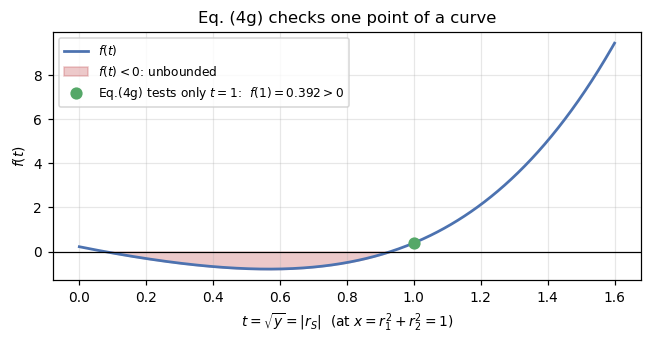
\includegraphics[width=0.82\textwidth]{figures/bfb_ft_curve.png}
\caption{The quartic \eqref{eq:ft} at the counterexample point \eqref{eq:badpoint}.
Eq.~(4g) tests only $t=1$, where $f(1)=0.392>0$ and the condition passes; the curve dips to
$-0.789$ at $t=0.565$, so the potential is unbounded below along a real neutral direction.}
\label{fig:ft}
\end{figure}

\subsection{An explicit counterexample}

At
\begin{equation}
\lambda=(1.8057,\,-1.8434,\,-1.5837,\,-1.5192,\,0.9116,\,1.0769,\,-0.1231,\,1.4658)
\label{eq:badpoint}
\end{equation}
all seven conditions Eq.~(4a)--(4g) are satisfied, yet along the unit direction
$$(r_1,r_2,r_S)=(-0.4598,\,-0.7944,\,0.3970)$$
one finds $V_4=-0.5074$, so $V_4\to-\infty$ as
the field norm grows. The closed-form minimum of \eqref{eq:ft} agrees with a direct scan to
four decimals: both give $-0.7891$ at $t=0.565$. This is checkable by hand in a few minutes,
which is why it is quoted in full.

\subsection{The corrected condition, and how much it removes}

Minimising \eqref{eq:ft} over $t\ge0$ in closed form (via the companion matrix of $f'$,
batched over parameter points) gives a condition that is exact on this slice. Its impact:

\begin{center}
\begin{tabular}{lrr}
\toprule
sample & Eq.~(4) survivors & removed by the corrected condition\\
\midrule
$3\times10^5$ points & $17\,277$ & $9.35\%$\\
$2\times10^6$ points & $114\,293$ & $9.47\%$\\
\bottomrule
\end{tabular}
\end{center}

Two independent samples, consistent. Validation: over 400 probe points the closed form and a
brute-force scan over $60\,000$ random directions give \emph{zero} disagreements about the
sign; at $40\,000$ directions both flag exactly the same 30 points. The closed form is not
finding artefacts, and the sampling is not missing violations at this resolution.

\subsection{Scope, stated honestly}

Condition \eqref{eq:ft} is exact on the \emph{real neutral} slice only. Complex-neutral and
charged directions are not covered analytically; the notebook handles them with a numerical
backstop over $40\,000$ directions in the full 12-dimensional field space, which removes a
further 3 points of the final 322. The residual gap is therefore real but small once the
other cuts are applied. Doing this properly --- separate analytic BFB-n and BFB-c
conditions --- is what \cite{BotoRomaoSilva22} does for $U(1)\times U(1)$,
$U(1)\times Z_2$ and $Z_2\times Z_2$; $S_3$ is not among their cases, and that is the
natural next piece of work.

\subsection{The caveat that governs everything above}
\label{sec:erratum}

\cite{DasDey14} carries an \textbf{Erratum, Phys.\ Rev.\ D \textbf{91}, 039905 (2015)},
which is \emph{not} posted to arXiv --- the arXiv record stops at v2 --- and is paywalled at
APS. Everything transcribed into our code therefore comes from the pre-erratum arXiv v2. The
erratum may already correct Eq.~(4g). What is established regardless is that the
\emph{arXiv-v2 conditions}, which are what \cite{GomezBock21}~\S2.2 delegates to and what the
community generally cites, are insufficient. Whether this is a new result or a rediscovery
of a known correction cannot be settled without reading that erratum
(\S\ref{sec:asks}).

\section{The scan}
\label{sec:scan}

Two million $\lambda$ points sampled uniformly on $U(-2,2)^8$ (seed \texttt{20260729}), with
$\theta$ scanned at $v=246$~GeV:

\begin{center}
\begin{tabular}{lrr}
\toprule
cut & surviving & of previous\\
\midrule
sampled                       & $2\,000\,000$ & ---\\
\cite{DasDey14}~Eq.~(4) bounded & $114\,293$ & $5.71\%$\\
$+$ corrected BFB \eqref{eq:ft} & $103\,465$ & $90.5\%$\\
$+$ tree unitarity              & $103\,465$ & $100.0\%$\\
$+$ no tachyons                 & $7\,608$   & $7.35\%$\\
$+$ $m_{H^\pm}>80$~GeV          & $6\,890$   & $90.6\%$\\
$+$ one CP-even at $125\pm3$~GeV & $322$     & $4.67\%$\\
\bottomrule
\end{tabular}
\end{center}

\begin{figure}[h]
\centering
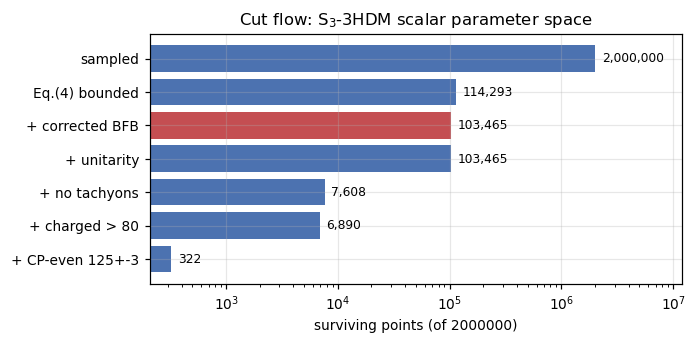
\includegraphics[width=0.78\textwidth]{figures/cut_flow.png}
\caption{Cut flow over the $2\times10^6$-point scan.}
\label{fig:cutflow}
\end{figure}

The line worth noticing is tree unitarity: it removes \textbf{nothing}. In this $\lambda$
range boundedness is the binding constraint, and unitarity would only bite at
$|\lambda|\gtrsim$ several --- at our old benchmark the largest eigenvalue was $3.63$
against the bound $16\pi\approx50.3$. This is worth knowing before spending effort on the
unitarity side.

\section{What the viable region looks like}
\label{sec:region}

\begin{figure}[h]
\centering
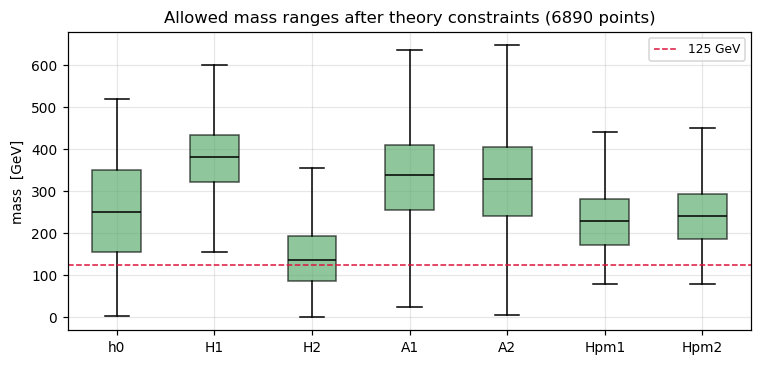
\includegraphics[width=0.80\textwidth]{figures/mass_ranges.png}
\caption{Allowed mass ranges for the seven physical scalars after all theory and
phenomenological cuts.}
\label{fig:masses}
\end{figure}

The surviving spectra cluster below a TeV, consistent with \cite{DasDey14}'s own conclusion
that many new scalars must be light. Five representative benchmark points, spanning the
viable range of the vacuum angle:

\begin{center}
\begin{tabular}{cccccccc}
\toprule
$\theta$ & $m_{h_0}$ & $m_{H_1}$ & $m_{H_2}$ & $m_{A_1}$ & $m_{A_2}$
& $m_{H^\pm_1}$ & $m_{H^\pm_2}$\\
\midrule
$0.206$ & $40$ & $406$ & $127$ & $414$ & $443$ & $183$ & $209$ \\
$0.651$ & $126$ & $295$ & $118$ & $345$ & $424$ & $115$ & $259$ \\
$0.811$ & $499$ & $356$ & $126$ & $137$ & $284$ & $304$ & $193$ \\
$1.421$ & $127$ & $304$ & $87$ & $481$ & $295$ & $135$ & $211$ \\
$1.493$ & $123$ & $539$ & $190$ & $435$ & $620$ & $422$ & $556$ \\
\bottomrule
\end{tabular}
\end{center}
{\small All masses in GeV. The $125\pm3$~GeV state is whichever CP-even scalar carries it ---
note it is $h_0$ in none of these, which is a coupling question the gauge sector settles, not
a mass-ordering one.}

\begin{figure}[h]
\centering
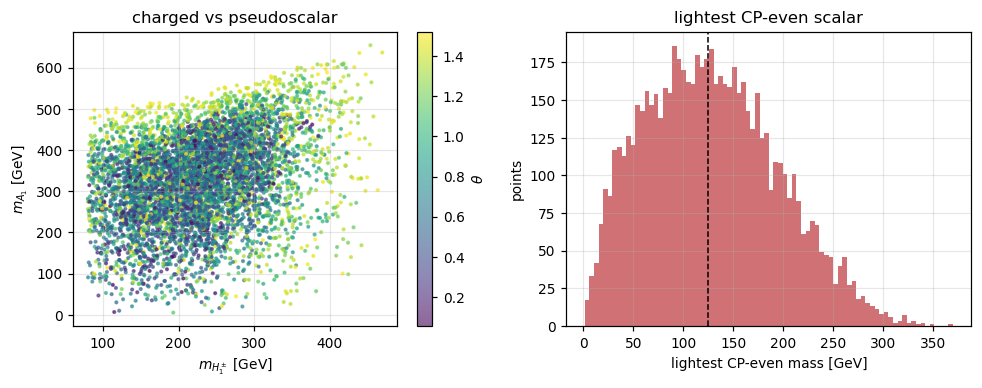
\includegraphics[width=0.92\textwidth]{figures/correlations.png}
\caption{Correlations across the viable region.}
\label{fig:corr}
\end{figure}

\clearpage
\section{Open questions, and what would help}
\label{sec:asks}

\begin{enumerate}\itemsep4pt
\item \textbf{Can you get the \cite{DasDey14} erratum?} Phys.\ Rev.\ D \textbf{91}, 039905
(2015). It is not on arXiv and I do not have APS access. This decides whether
\S\ref{sec:main} is a new result or a rediscovery, and it may also touch the tree-unitarity
eigenvalues of Eq.~(37), which we currently check only for internal consistency and cannot
check against a corrected source. This is the single most useful thing.

\item \textbf{Cross-check the unitarity bounds against \cite{BentoRomaoSilva22}}, which
recomputes them for all symmetry-constrained 3HDMs and post-dates the erratum. That would
close the unitarity question independently of the erratum.

\item \textbf{Complete the boundedness analysis} for complex-neutral and charged directions,
following \cite{BotoRomaoSilva22}'s method. $S_3$ is not among the cases they treat.

\item \textbf{Is any of \S\ref{sec:main} worth writing up separately}, or does it belong as a
section of the LFV paper? It concerns a constraint the 3HDM literature uses widely, so my
instinct is that it stands alone --- but that depends on the erratum.
\end{enumerate}

\appendix
\section{The derivation ledger}

Each derived step in the notebook records what was claimed, whether it was derived here or
imported, which independent checks it survived, and what would falsify it. The full typeset
version is the companion document \texttt{derivations\_01.tex}; in summary:

\begin{center}
\begin{tabular}{p{0.30\textwidth}p{0.13\textwidth}p{0.47\textwidth}}
\toprule
claim & status & independent checks\\
\midrule
The $(a\ldots h)\leftrightarrow\lambda$ dictionary, $e=-\lam4$ & derived &
solved from an over-determined system, not guessed; the four solved entries agree with
term matching; $e=+\lam4$ fails all four published masses; the sign question vanishes as
$\lam4\to0$\\
\addlinespace
The real neutral slice, and the absence of $\lam2$ & derived &
degree-4 homogeneous; the cubic covariant is $\mathbb Z_3$-invariant (the check was
falsified on a broken sign, so it has teeth); $\lam4\to0$ reduces to a quadratic form;
an independent $r_2=0$ hand slice reproduces it\\
\addlinespace
\cite{DasDey14}~Eq.~(4a)--(4g) & \textbf{imported} &
tested directly against our own $V_4$: counterexamples found\\
\addlinespace
The exact boundedness condition \eqref{eq:ft} & derived &
agrees with $60\,000$-direction brute force on every probe point; Eq.~(4g) is exactly
$f(1)>0$\\
\bottomrule
\end{tabular}
\end{center}

\begin{thebibliography}{9}

\bibitem{DasDey14} D.~Das and U.~K.~Dey,
\emph{Analysis of an extended scalar sector with $S_3$ symmetry},
Phys.\ Rev.\ D \textbf{89}, 095025 (2014),
\href{https://arxiv.org/abs/1404.2491}{arXiv:1404.2491},
\href{https://doi.org/10.1103/PhysRevD.89.095025}{doi:10.1103/PhysRevD.89.095025}.
Erratum: Phys.\ Rev.\ D \textbf{91}, 039905 (2015) --- not posted to arXiv; everything used
here comes from arXiv v2.

\bibitem{GomezBock21} M.~Gómez-Bock, M.~Mondragón and A.~Pérez-Martínez,
\emph{Scalar and gauge sectors in the 3-Higgs Doublet Model under the $S_3$-symmetry},
Eur.\ Phys.\ J.\ C \textbf{81}, 942 (2021),
\href{https://arxiv.org/abs/2102.02800}{arXiv:2102.02800},
\href{https://doi.org/10.1140/epjc/s10052-021-09731-3}{doi:10.1140/epjc/s10052-021-09731-3}.

\bibitem{BentoRomaoSilva22} M.~P.~Bento, J.~C.~Romão and J.~P.~Silva,
\emph{Unitarity bounds for all symmetry-constrained 3HDMs},
JHEP \textbf{08} (2022) 273,
\href{https://arxiv.org/abs/2204.13130}{arXiv:2204.13130},
\href{https://doi.org/10.1007/JHEP08(2022)273}{doi:10.1007/JHEP08(2022)273}.

\bibitem{BotoRomaoSilva22} R.~Boto, J.~C.~Romão and J.~P.~Silva,
\emph{Bounded from below conditions on a class of symmetry constrained 3HDM},
Phys.\ Rev.\ D \textbf{106}, 115010 (2022),
\href{https://arxiv.org/abs/2208.01068}{arXiv:2208.01068},
\href{https://doi.org/10.1103/PhysRevD.106.115010}{doi:10.1103/PhysRevD.106.115010}.

\end{thebibliography}

\end{document}
